\documentclass[12pt]{article}
\usepackage[a4paper, total={6in, 9in}]{geometry}
\usepackage{graphicx}
\graphicspath{ {./images/output/} }
\usepackage{caption}
\usepackage[english]{babel}
\usepackage{titling}
\usepackage{float}
% \usepackage{amsmath}
% \usepackage{minted}
% \usepackage{multicol}
% \usepackage{array}
% \usepackage{setspace}
% \usepackage{placeins}
\setlength{\parindent}{0pt}

% \usepackage{lipsum}

\title{Designing a Ladder Circuit Diagram}
\author{}
\date{}

\pagenumbering{gobble}
\begin{document}
\vspace*{\fill}
\begin{center}

    \emph{Heaven's Light is Our Guide} \\
    \textbf{Rajshahi University of Engineering and Technology} \\

    \begin{figure}[H]
        \centering
        
\includegraphics[scale=.34]{images/RUET_logo.png}
        \label{fig:ruet_logo}
    \end{figure}
    \vspace{5mm}

    \textbf{Course Code}\\
    ECE 3200\\
    \vspace{3mm}
    \textbf{Course Title}\\
    Electrical Services Design

    \vspace{5mm}
    \textbf{Experiment Date:} {February 4, 2025}\\
    \textbf{Submission Date:} {February 18, 2025}\\

    \vspace{5mm}
    \textbf{Lab Report 5: \\ Implementation of Parametric \& Full Units PLC: Insertion, Editing, \& Modification.}

    \vspace{15mm}

    \begin{tabular}{c|c}
        \textbf{Submitted to} & \textbf{Submitted by} \\
        Md. Faysal Ahamed     &                       \\
        Lecturer              &                       \\
        Dept of ECE, RUET     & Md. Tajim An Noor     \\
        -                     & Roll: 2010025         \\
        Moloy Kumar Ghosh     &                       \\
        Lecturer              &                       \\
        Dept of ECE, RUET     &                       \\
    \end{tabular}

\end{center}
\vspace*{\fill}


\pagebreak

\tableofcontents

\pagebreak
\pagenumbering{arabic}
\maketitle

\section*{Introduction}
\addcontentsline{toc}{section}{Introduction}
A ladder circuit, also known as a ladder logic diagram, is a graphical representation of an electrical control system. It resembles the rungs of a ladder, hence the name. Each rung represents a control operation, typically involving relays, switches, and other control devices. Ladder diagrams are widely used in industrial control applications to design and document the logic of programmable logic controllers (PLCs). They provide a clear and intuitive way to visualize the sequence of operations and the interactions between different components in the control system.
\\\\
In this experiment, a ladder circuit diagram was designed using AutoCAD Electrical. The primary objective was to familiarize ourselves with the software and its various functions. The focus was on creating the diagram without performing any simulations. This exercise helped in understanding the capabilities of AutoCAD Electrical in designing electrical circuits and the importance of accurate diagramming in electrical engineering.

\section*{Required Equipment/Software}
\addcontentsline{toc}{section}{Required Equipment/Software}
\begin{itemize}
    \item AutoCAD Electrical
\end{itemize}

\section*{Procedure}
\addcontentsline{toc}{section}{Procedure}
\begin{enumerate}
    \item \textbf{Launch AutoCAD Electrical:} Open the AutoCAD Electrical software on your computer.
    \item \textbf{Create a New Project:} Go to the 'Project Manager' and create a new project. Name the project appropriately.
    \item \textbf{Insert a New Drawing:} Within the project, insert a new drawing. Set the drawing properties such as the title block and template.
    \item \textbf{Set Up the Drawing Environment:} Configure the drawing environment by setting the appropriate layers, line types, and colors.
    \item \textbf{Draw the Ladder Rungs:} Use the 'Ladder' tool to draw the vertical and horizontal lines that form the rungs of the ladder diagram.
    \item \textbf{Insert Components:} Place the necessary electrical components such as relays, switches, and contacts onto the rungs using the 'Insert Component' tool.
    \item \textbf{Connect Components:} Draw the connections between the components using the 'Wire' tool. Ensure that all connections are accurately represented.
    \item \textbf{Annotate the Diagram:} Add labels, descriptions, and other annotations to the diagram to provide clarity and additional information.
    \item \textbf{Verify the Diagram:} Double-check the diagram for accuracy and completeness. Ensure that all components and connections are correctly represented.
    \item \textbf{Save and Print:} Save the completed ladder diagram and print it if necessary for documentation or presentation purposes.
\end{enumerate}

\section*{Output}
\addcontentsline{toc}{section}{Output}
\begin{figure}[H]
    \centering
    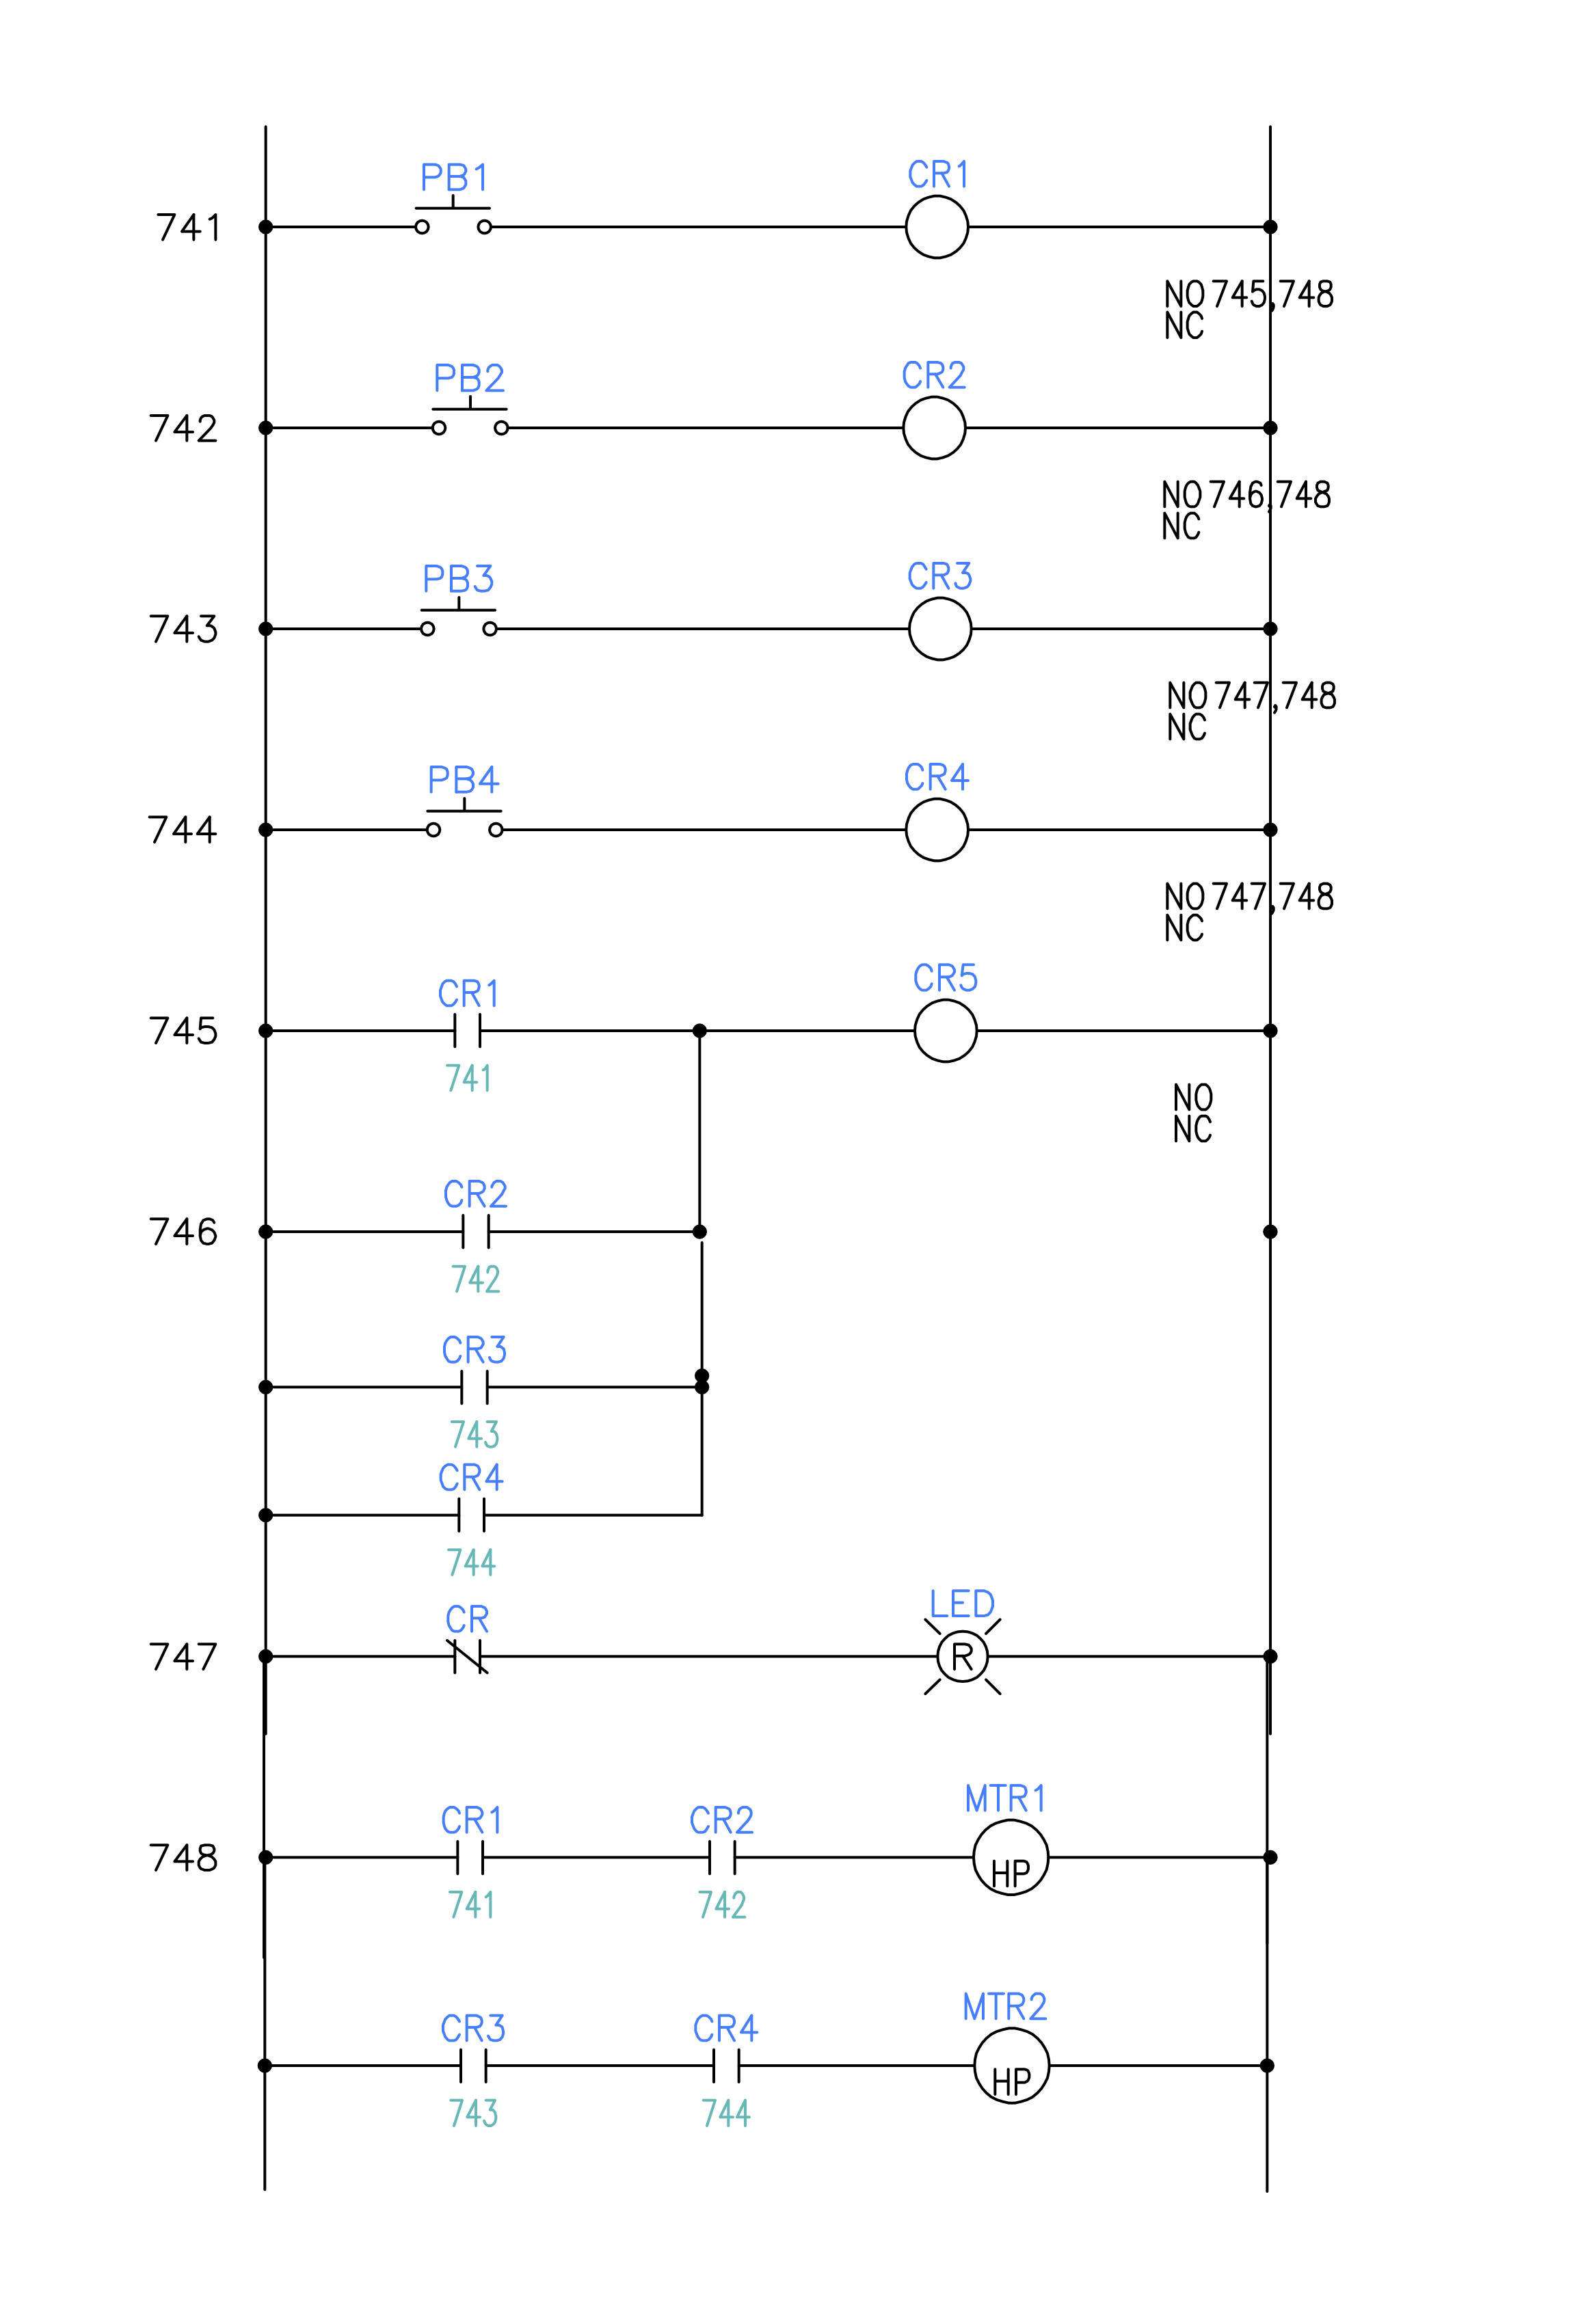
\includegraphics[width=.9\textwidth]{ladder.png}
    \caption{Ladder Circuit Diagram created using AutoCAD Electrical}
    \label{fig:ladder_circuit}
\end{figure}

\section*{Discussion \& Conclusion}
\addcontentsline{toc}{section}{Discussion \& Conclusion}
The ladder circuit diagram was successfully designed using AutoCAD Electrical. The process included launching the software, creating a new project, setting up the drawing environment, and inserting and connecting components. Each step ensured the accuracy and completeness of the final diagram. Proper planning and organization, such as setting up the drawing environment correctly and using appropriate layers, line types, and colors, were essential in creating a clear and organized diagram. Annotations and labels provided additional clarity, making the diagram easier to understand.

% \bibliographystyle{IEEEtran}
% \renewcommand{\bibname}{References}
% \addcontentsline{toc}{section}{References}
% \bibliography{ref}

\end{document}
